\documentclass[class=report, crop=false]{standalone}
\usepackage[subpreambles=true]{standalone}
\usepackage{import}
\usepackage{amsmath}

\begin{document}
The recovery system's job is to provide safe descent and to allow the ground crew to locate the craft. \\
The system consists of a steerable parachute and a GPS device that gives the ground crew the position of the satellite. 
The parachute is the main component of the GlideCan system, while the GPS module is a crucial part of the SatTrack system. \\

To achieve a parachute with the desired properties (vertical speed and horizontal speed) we have tried two seperate approaches. One of them was to create a ram-air parachute (flying wing design) and the other one was to create an asymetrical dome-shaped parachute. \\
In the first design, we wanted to base our parachute on military grade gliding crafts. We've then settled on creating and designing a ram-air parachute. A ram air design is composed of wing shaped cells sewn together, the cells being made out of a durable and elastic material (In our case, we used ripstop nylon). \\
The characteristics of the first prototype were as follows: \\
\begin{minipage}{.34\textwidth}
  \begin{tabular}{|c|c|}
    \hline
    Profile & NACA 4418 \\\hline
    Elongation & $2:1
    $ \\\hline
    Area & $670\text{cm}^2$ \\\hline
  \end{tabular}
\end{minipage}
\hfill
\begin{minipage}{.66\textwidth}
  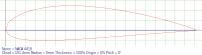
\includegraphics[width=\textwidth]{ext/parachuteprofile.pdf}
\end{minipage}
\\\newpage
\vfill
We planned for the parachute to work by creating most of the force needed to keep the satellite midair from its aerodynamical lift.
A theoretical model showed that with $6\frac{\text{m}}{\text{s}}$ of progressive movement the lift equalizes the weight of the system. \\
Sadly however, the test of our prototype revealed some critical flaws with the design.
The most crippling was the inability of the parachute to inflate and keep the desired shape in flight.
The descent speed was also around $9\frac{\text{m}}{\text{s}}$, which was too fast for our needs.
We are thinking about tweaking the design, by increasing the height of the cells or adding extra area on the sides of the parachute. \\
The secondary design was developed as a backup plan after the former one didn't meet our expectations. \\
The second design is a modified regular parachute with holes cut on one side of it.
These holes are not symetrical so as to cause the parachute to traverse in one direction.
We've decided to get a copular parachute with a radius of 27.5cm. We are aware that this is an overkill, but the holes on the sides should compensate the excess area. \\

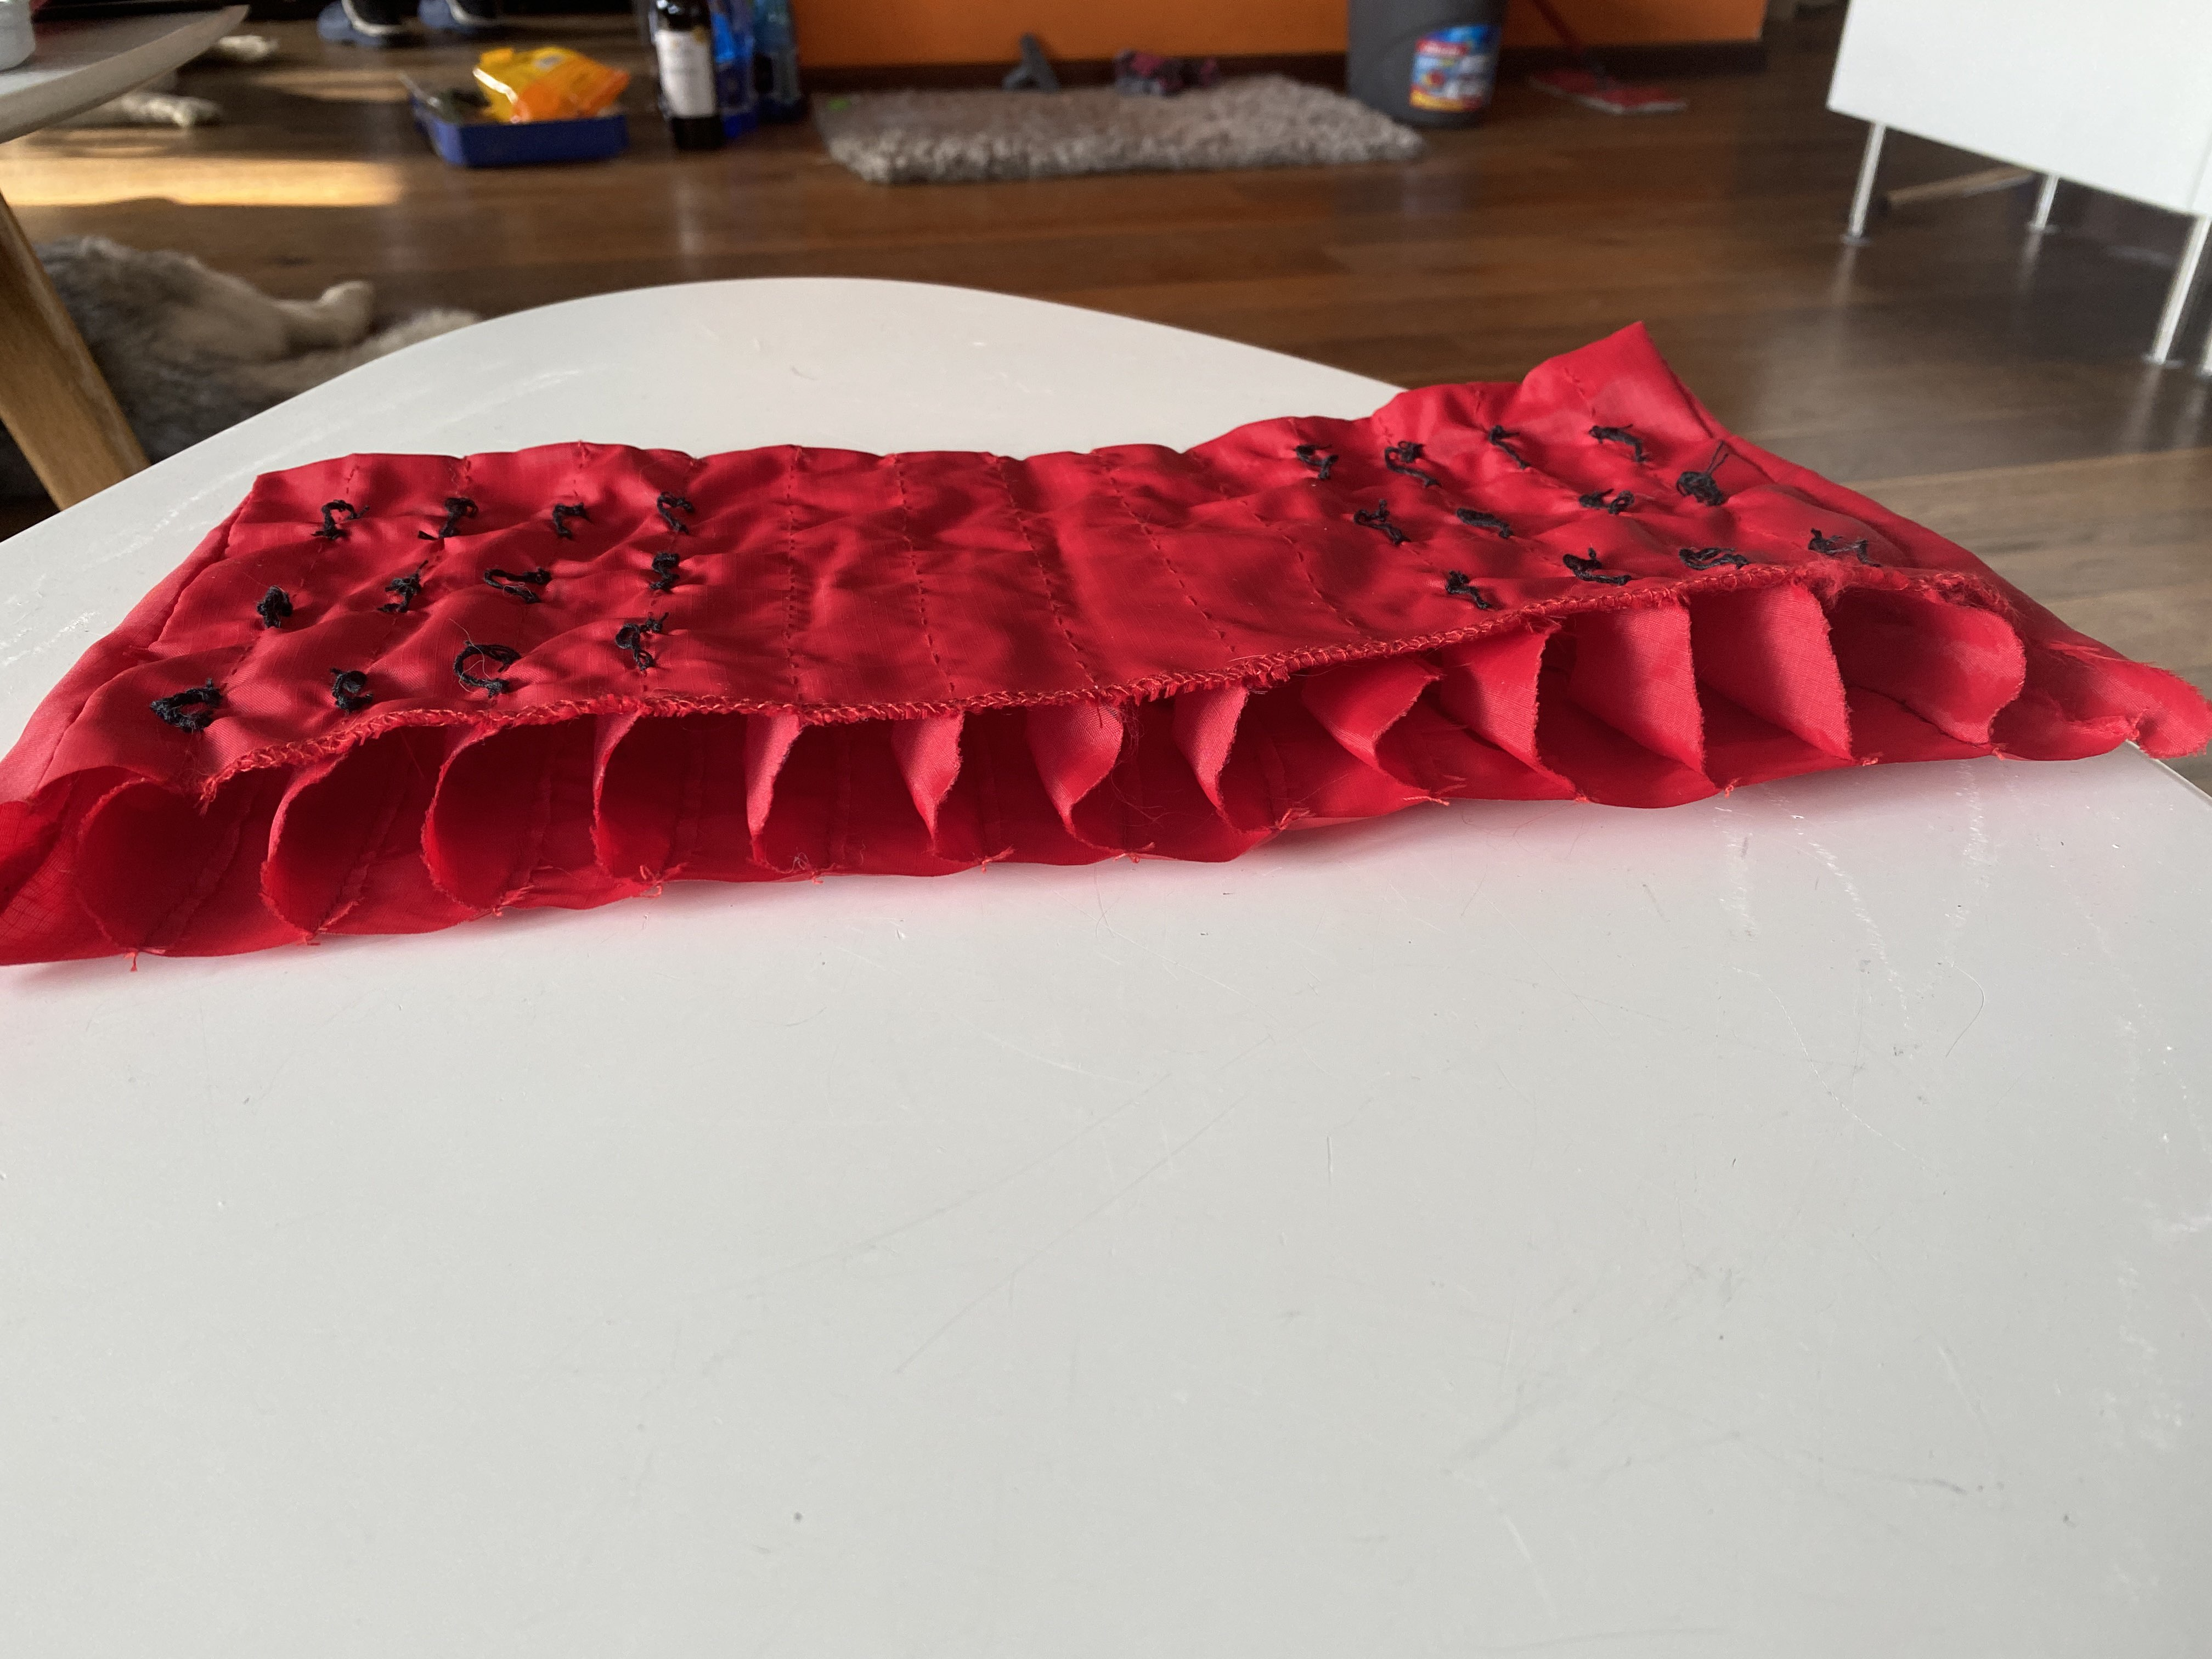
\includegraphics[width=\columnwidth]{ext/parachutefirst.png}
\captionof{figure}{The primary design}

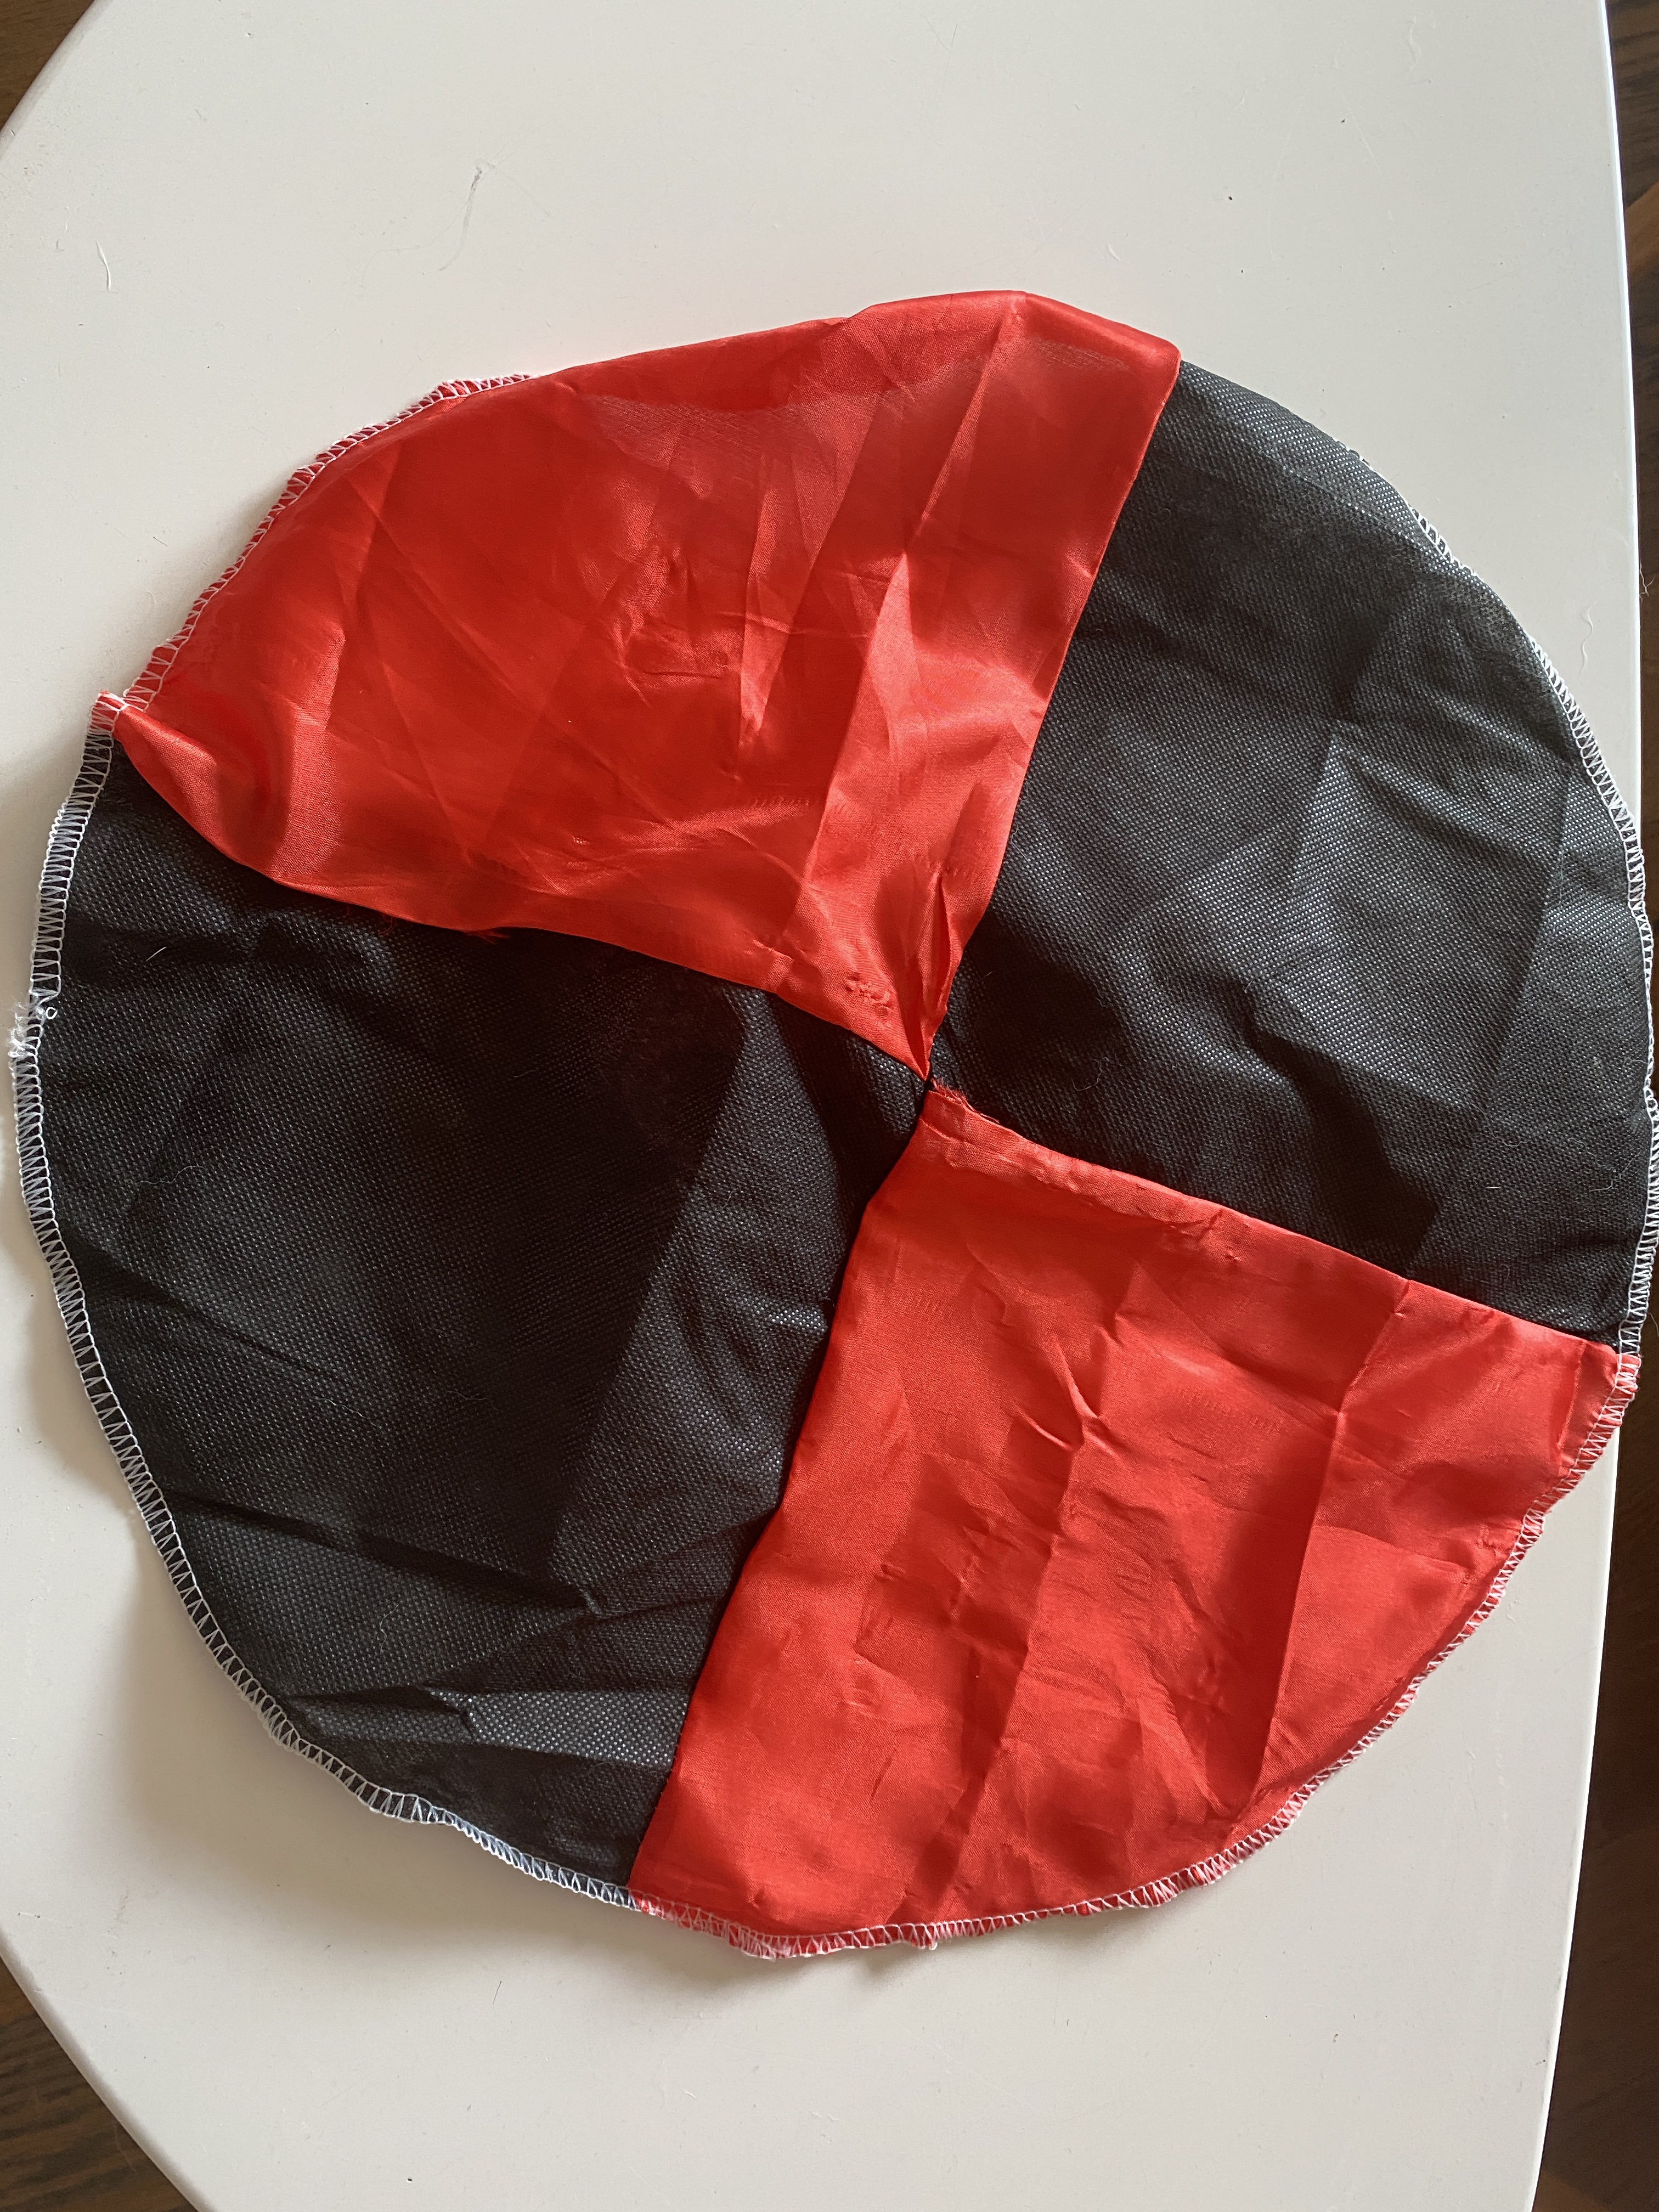
\includegraphics[width=\columnwidth]{ext/parachutesecond.png}
\captionof{figure}{The secondary design}

\vfill

\end{document}
